\subsection{Deliberate undersampling and recovery}
The controlled failure bypasses anti-alias filtering at 8 kHz, against
the selected 16 kHz path. Removing 6 kHz before sampling would test content
loss instead of folding. No stochastic degradation or quantisation is used.
\begin{equation}
 x_{16}[m]=x_{\mathrm{ref}}[3m],\qquad
 x_8[m]=x_{\mathrm{ref}}[6m].
 \label{eq:r13-samples}
\end{equation}
Both last 2 s, with 0.5 Hz bin spacing. The mathematical prediction precedes
sample/spectrum checks:
\begin{equation}
 f_d=f_0-qf_s\in[-f_s/2,f_s/2),\qquad f_a=|f_d|,
 \label{eq:signed-alias}
\end{equation}
The implementation is $ f_d=((f_0+f_s/2)\bmod f_s)-f_s/2 $.
At 8 kHz, 6000 Hz maps to $-2000 $ Hz; its positive 2 kHz cosine phase changes
from $-\pi/2 $ to $+\pi/2 $ (Eq.~\eqref{eq:alias-phase}). The 440/1320/2200 Hz
tones remain distinct, with no collisions or endpoint ambiguities.

\begin{table}[!htbp]
 \centering
 \caption{Predicted/detected 8 kHz peaks; phase is in units of $\pi $. The 6 kHz source folds to positive 2 kHz with reversed cosine phase.}
 \label{tab:alias-mapping}
 \begin{tabular}{rrrrrr}
\toprule
Source (Hz) & Signed (Hz) & Predicted (Hz) & Measured (Hz) & Amplitude & $\phi/\pi$ \\
\midrule
440 & 440 & 440 & 440 & 1.0 & -0.500 \\
1320 & 1320 & 1320 & 1320 & 0.6 & -0.500 \\
2200 & 2200 & 2200 & 2200 & 0.3 & -0.500 \\
6000 & -2000 & 2000 & 2000 & 0.1 & 0.500 \\
\bottomrule
\end{tabular}

\end{table}

% Keep the measured-peak result paragraph intact across the table/figure stack.
\noindent\begin{minipage}{\linewidth}
Peaks are detected with the same $-60 $ dB local-maximum rule, rather than
declared measured by selecting predicted bins. Normalised complex
coefficients and wrapped phases are also checked; all 16 checks pass.
Both paths use the same Fourier recovery and all original grid positions.
The 8 kHz MSE/RMSE/NMSE/peak error are $\UnderMse $, $\UnderRmse $,
$\UnderNmse $ and $\UnderMaxError $; the 16 kHz MSE is $\AliasBaselineMse $.
\end{minipage}\par

\begin{figure}[!htbp]
 \centering
 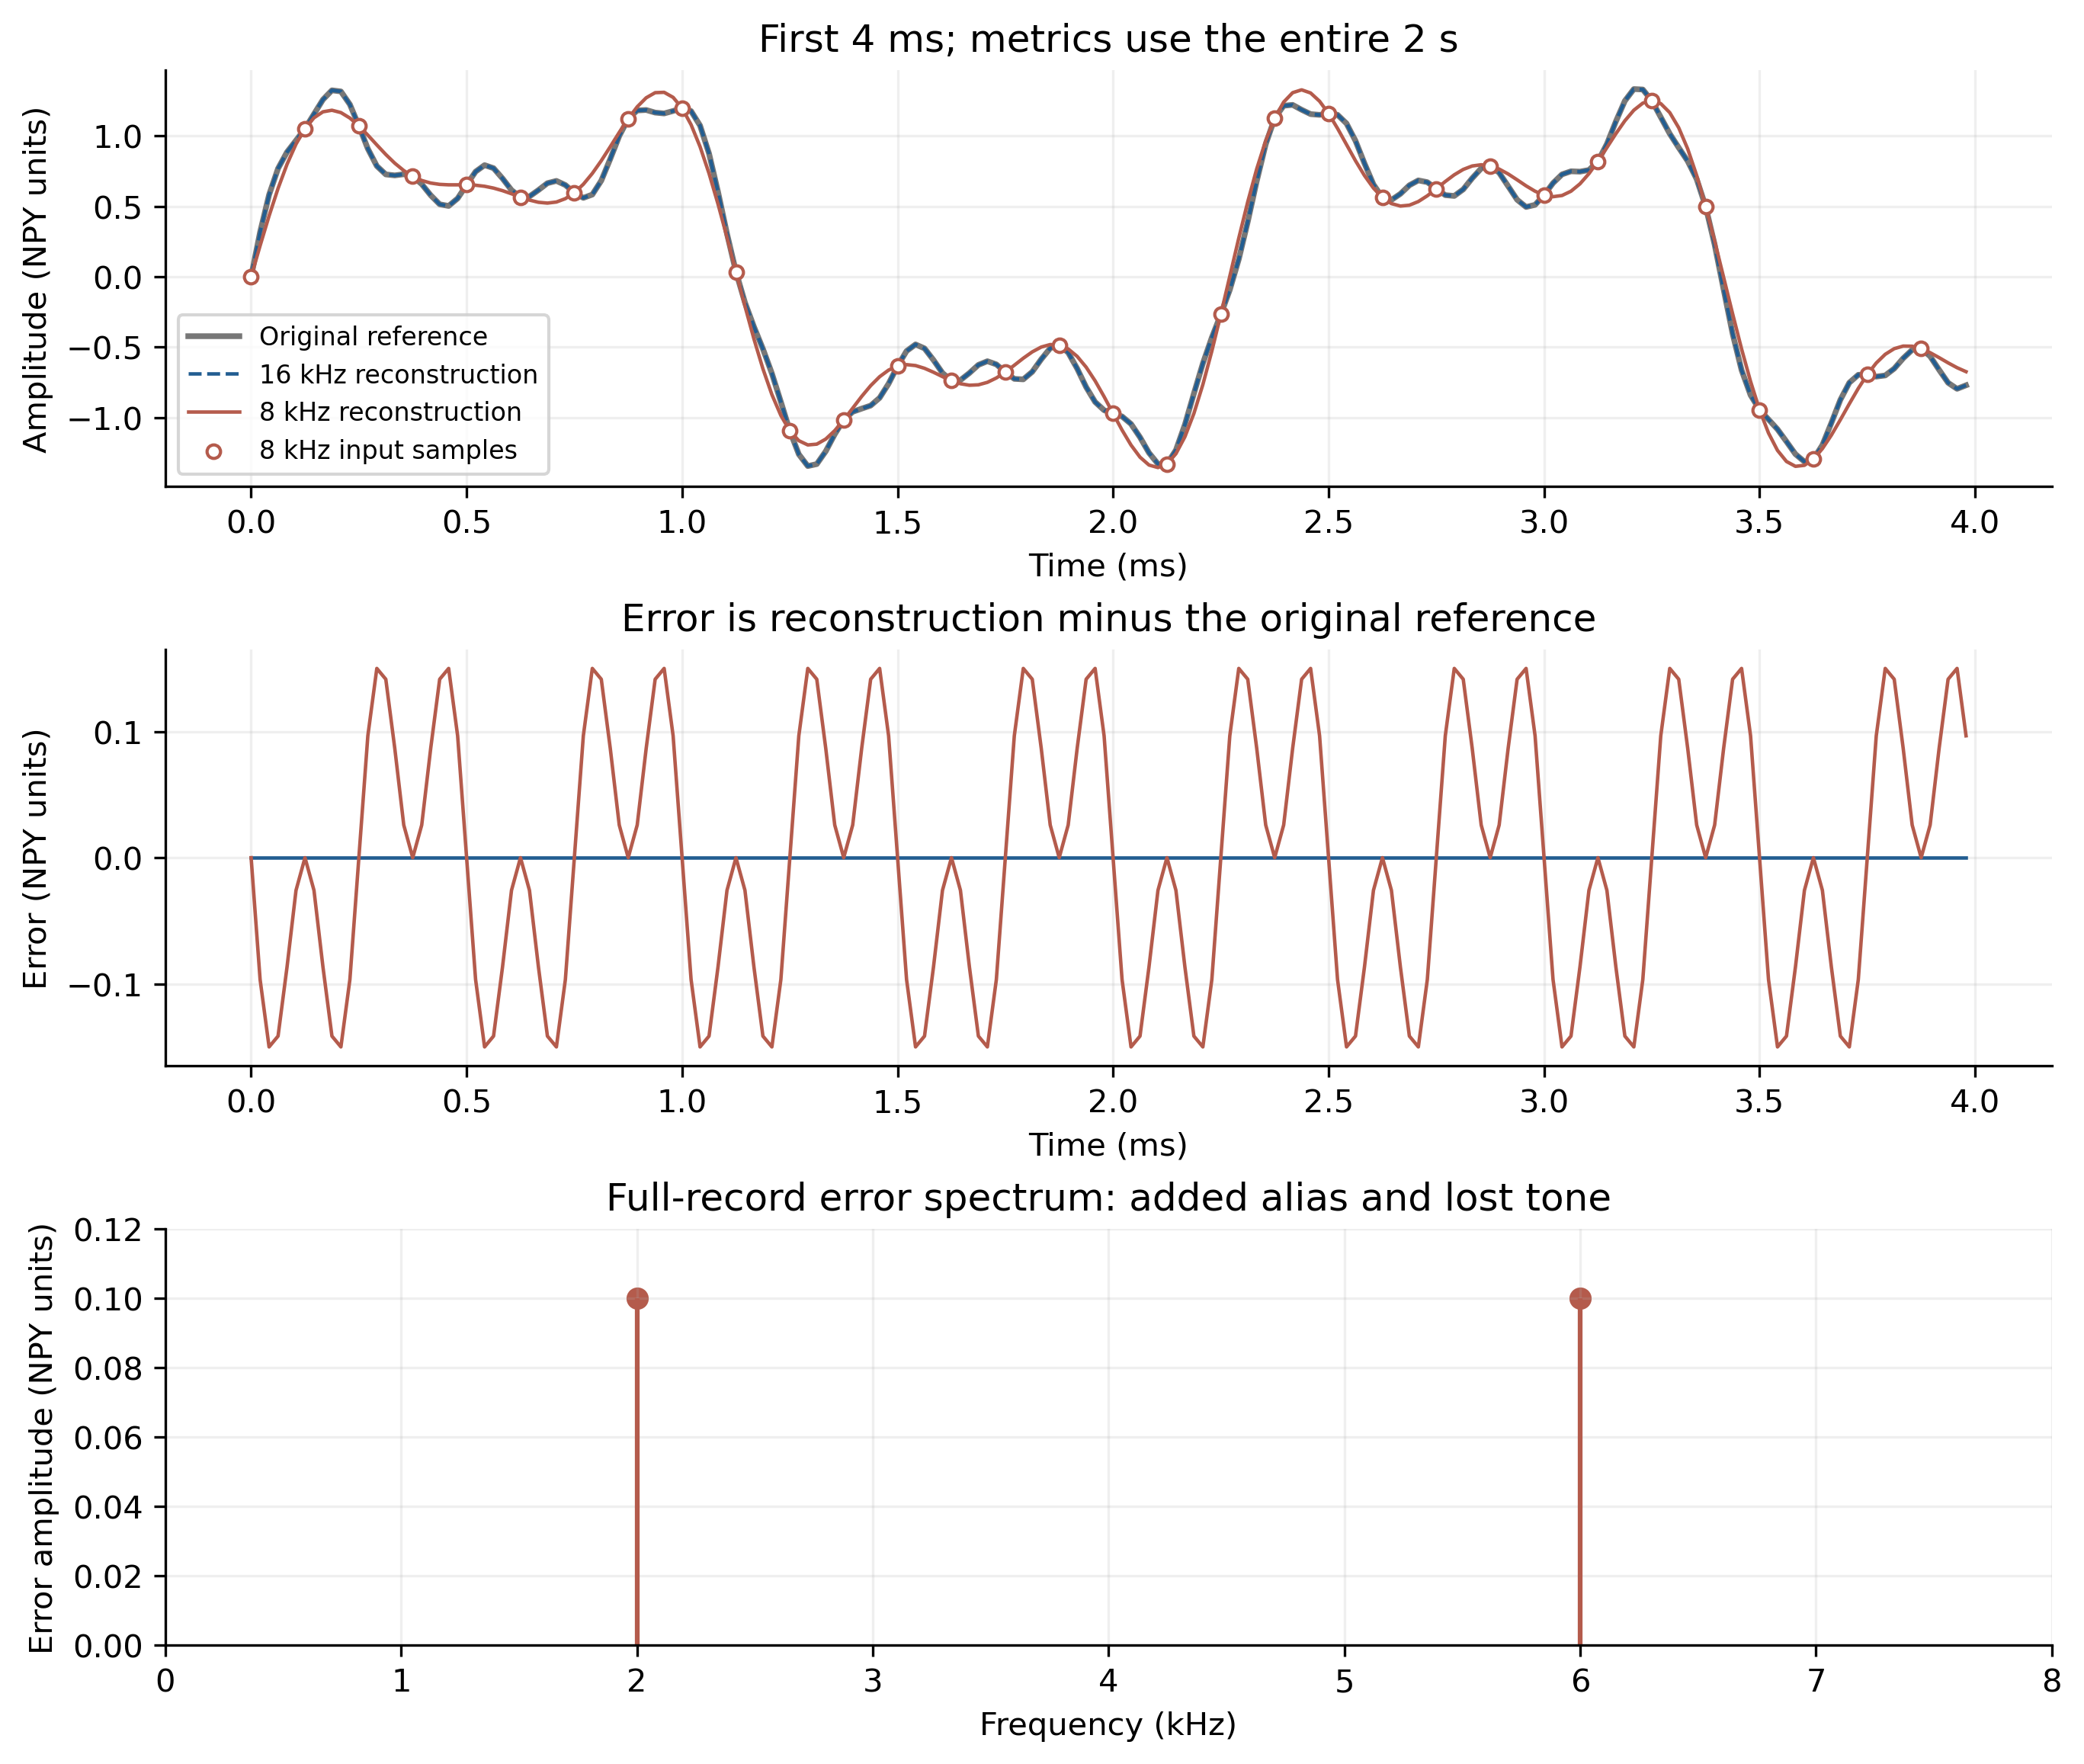
\includegraphics[width=.76\linewidth]{images/aliasing_reconstruction_error.png}
 \caption{Recovery and error: first 4 ms waveforms above, full 2 s error spectrum below. All 96000 positions enter the reported MSE; sample fitting alone does not identify the source.}
 \label{fig:alias-recovery}
\end{figure}

% Keep this result paragraph together if the preceding figure moves to a page top.
\noindent\begin{minipage}{\linewidth}
Both recoveries fit their own samples to about $10^{-15}$, demonstrating
that sample fitting does not identify the source. The phase-aware error
model predicts 0.1-amplitude tones at 2/6 kHz and MSE 0.01
(Eqs.~\eqref{eq:alias-error-model}--\eqref{eq:alias-error-power}); the
full-record error spectrum agrees. This explanation is not information
supplied to recovery. Complex coefficients must be added before power
when aliases coincide. Later filtering/coding cannot resolve this
ambiguity without extra source information.
\end{minipage}\par
